\documentclass[12pt, french]{article}
\usepackage{fontspec}
\setmainfont{Arial}
\usepackage{setspace}
\singlespacing

\usepackage{graphicx}
\usepackage{caption}
\usepackage[T1]{fontenc}
\usepackage[utf8]{inputenc}
\usepackage{lmodern}
\usepackage{geometry}
\geometry{
	a4paper,
	left=20mm,
	right=20mm,
	top=25mm,
	bottom=25mm,
}

\usepackage{pgfgantt}
\usepackage{eurosym}

%\usepackage[babel=true, kerning=true]{microtype}

\usepackage{subcaption}

\usepackage[unicode=true,pdfusetitle,bookmarks=true,bookmarksnumbered=false,bookmarksopen=false,
breaklinks=false,pdfborder={0 0 0},backref=false,colorlinks=true,urlcolor=blue]{hyperref}

\graphicspath{{images/}}

\author{Andrea Brugnoli \\ 
\hspace{2.8pt} Docteur ISAE-Supaéro 2020\\
Ingénieur ISAE-Supaéro 2017}
\title{Project MORPHEUS \\
\vspace{.3cm}
\Large{Model Order Reduction for multi-PHysical and Energy-Unified Systems}  }

\date{}

\begin{document}

\maketitle

\large{Dossier de candidature au prix de la fondation Jean-Jacques et Félicia
	Lopez-Loreta pour l'excellence académique.}


\begin{figure}[h]
	\centering
	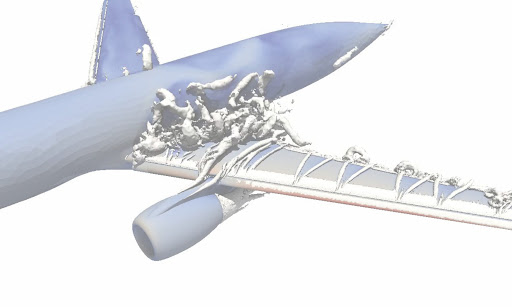
\includegraphics[width=.95\textwidth]{3Dplane.jpg}
	\captionsetup{labelformat=empty}
	\caption{Source: \href{http://www.fenics-hpc.org/}{FEniCS-HPC website}}
\end{figure}





\thispagestyle{empty}

\newpage

\section{Résume du projet}

Le but du projet MORPHEUS consiste à mettre en place des méthodes numériques
pour accélérer la simulation des problèmes d'interaction fluide-structure (IFS), par rapport au temps de calcul requis pour une simulation haute-fidélité. Il sera donc possible d’intégrer des modèles plus économiques, qui pourront remplacer des simulations très coûteuses, et ainsi de faciliter le design et la prise de décisions. A la différence de plusieurs méthodes proposées dans la littérature, l'impératif est la fidélité à la structure physique du problème.  Cette structure est le plus souvent ignorée par les algorithmes de réduction, qui traitent les simulations comme des boîtes noires. Les modèles réduits respectueux de la physique sont beaucoup plus précis que ceux qui ne la garantissent pas et leur utilisation pourra radicalement améliorer les techniques normalement utilisées pour la réduction des modèles et l’optimisation. Pour realiser son ambition, ce projet vise à utiliser des formalismes mathématiques récents pour la modélisation multiphysique et la digitalisation des modèles. Les outils capables de prédire précisément le comportement des systèmes complexes ont une importance fondamentale pour nous aider à affronter les prochains défis technologiques et sociétaux. Le fait que cette année le Prix Nobel de Physique ait été attribué à trois chercheurs travaillant sur ce sujet\footnote{\url{https://www.nobelprize.org/prizes/physics/2021/summary/}} confirme
l’importance et l'actualité de cet axe de recherche.


\section{Développement du projet scientifique}

\subsection{Les problèmes multiphysiques}
L'ingénierie computationnelle est une science récente, multidisciplinaire et en expansion rapide. Son but consiste à mettre en place des modèles mathématiques et numériques pour prédire le comportement des systèmes complexes. Cela permet d'éviter l'utilisation des tests expérimentales très couteaux pour les systèmes en phase de conception et de détecter de fautes pendant le cycle de vie des composants. Ce domaine est en expansion rapide car aujourd'hui on dispose des ordinateur plus puissant et surtout parce que, grâce au développement des codes open source, les logiciels des calcul sont beaucoup plus accessibles, robustes et faciles à utiliser. Toutefois les problèmes multiphysique, qui sont centrales dans les applications industrielles, sont extrêmement compliqués à traiter. Cela est d\^u d'une part à la difficulté associé au traitement des différentes physique et d'autre part à la taille des systèmes obtenus, qui nécessitent des plusieurs jours, voir plusieurs semaines, pour être résolu à l'aide d'un supercalculateur \cite{keyes2013}. Ces problématiques posent des barrières pour l'utilisation des modèles numériques en industrie. 


\subsection{Outils scientifiques du projet Morpheus}

\paragraph{\large Un formalisme unifiant pour la modélisation des systèmes dynamiques\\}
Un formalisme mathématique très prometteur pour traiter les problèmes multiphysique est le formalisme port-Hamiltonienne \cite{vanderSchaft2002}, basé sur la mécanique Hamiltonienne et les graphes de liaisons pour la modélisation des systèmes dynamiques. Au c\oe{}ur de ce formalisme il y a l'idée que tout système physique peut être décrit d'une manière modulaire, c'est a dire à partir des ses composant simples, qui interagissent entre eux et avec le milieu environnant à travers des portes. Les portes d'interactions contiennent l'information relative au flux d'énergie entre les différents composants et entre différents domaines physiques (mécanique, électromagnétisme ou fluidodynamique). La conception modulaire est fondamentale dans l'ingénierie, car le design de tout système technologique est fait à partir des éléments simples qui sont assemblés pour donner lieu à la complexité qui nous entoure. Prenez par exemple un avion, un hélicoptère, un satellite (cf. Fig. \ref{fig:satellite}) ou un téléphone portable : pour pouvoir optimiser leur design il est indispensable de disposer d'un outil de modélisation capable de décomposer la complexité d'une manière à retrouver les différents composants clés.

\begin{figure}[tb]
	\centering
	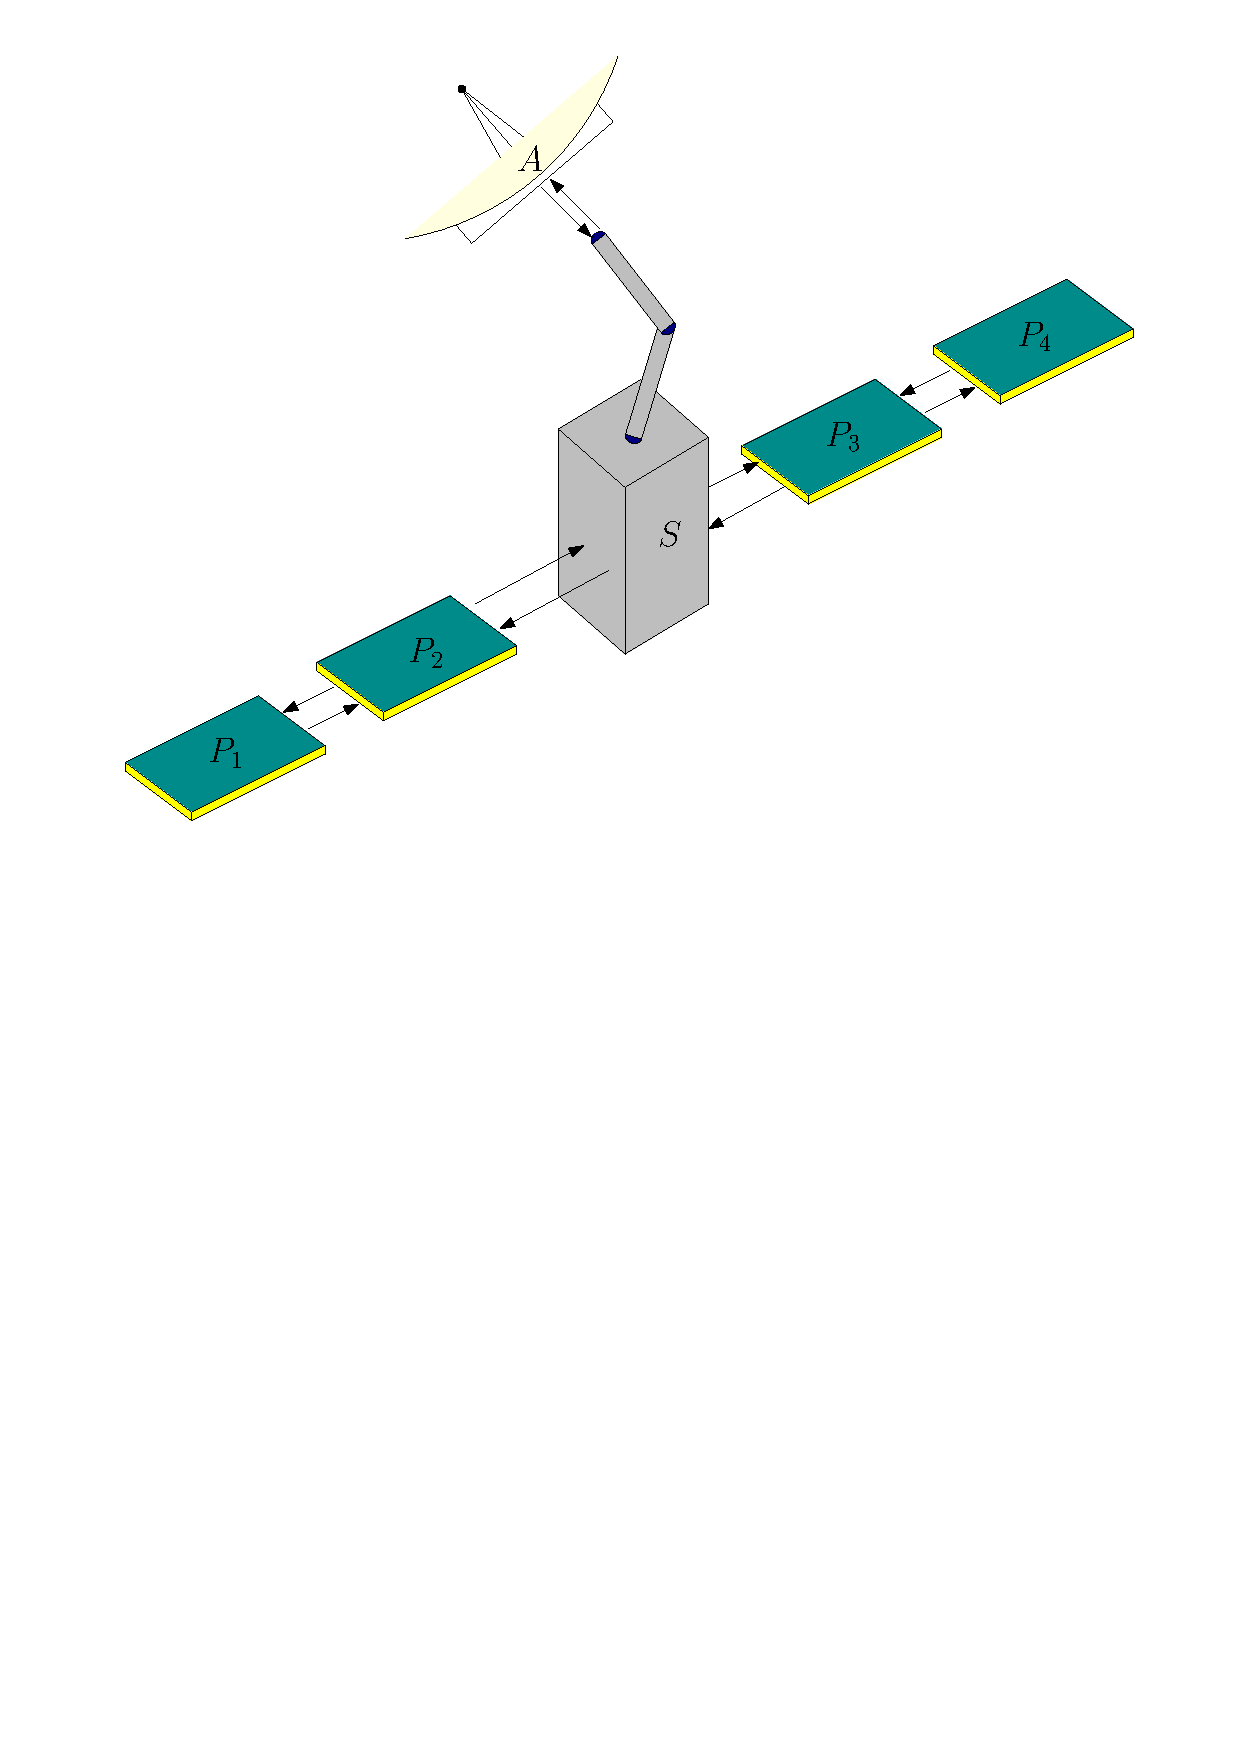
\includegraphics[width=.6\textwidth]{satellite.pdf}
	\caption{Schéma modulaire représentant un satellite de télécommunication.}
	\label{fig:satellite}
\end{figure}

\paragraph{\large Une methodologie structurée pour la discretisation des EDP\\}
Les algorithmes numériques utilisés en industrie sont adaptés à la nature physique du problème. Pour la mécanique la méthode des éléments finis est privilège par les ingénieur. Pour la fluidodynamique, les volumes finis sont majoritairement utilisés car il garantissent le respect des lois de conservation. Quand il faut utiliser ces deux approches simultanément, par exemple pour traiter des problèmes couplés, leur couplage pose plusieurs challenges. Les deux méthodes utilisent des dégrées de liberté différents (i.e. différents entités topologique du maillage) et l'interconnexion introduit forcement des erreurs. Un outil de modélisation général nécessite d'une méthode de discrétisation également générale, capable de  garantir la possibilité d'interconnecter des physiques distinctes. Ce formalisme unifiant, la méthode des éléments finis en calcul extérieur or FEEC\footnote{Le calcul extérieur représente une généralisation du calcul vectorielle basée sur la géométrie différentielle.},  à été développé récemment \cite{arnold2006acta}. Cette théorie mathématique à permis des développement importants pour la discrétisation des équation à dérivées partielles issues de la physique. Elle à été appliqué avec succès au cas de la mécanique des solides, la fluidodynamique et l'électromagnétisme et elle représente un outil puissant pour les application multiphysique. 

\paragraph{\large L'intelligence artificielle pour obtenir des modeles reduits\\}
Toute méthode de discrétisation, même les plus sophistiquées, amène à des systèmes dont la taille dépasse facilement le million d'inconnus. Pour pouvoir optimiser le design des composantes mécaniques, il faut simuler ces modèles plusieurs fois. Cela amène à des coûts computationnelles prohibitifs même pour les entreprises dotés de plus avancés centres de calcul. Il est donc indispensable d'introduire des méthodes de réduction, qui sont sensé construire un modèle plus simple, capable néanmoins de retenir les propriétés principales du système de départ. La grande majorité de ces méthodes supposent que l'on puisse obtenir un système réduit à travers une méthode essentiellement linéaire, i.e. la Décomposition Orthogonale en Valeurs Propres (POD) \cite{shinde2019,tello2020fluid}. Cette hypothèse n’est pas valable pour tout système exhibant un comportement non-linéaire et conduit à surestimer la dimension du système réduit. Grâce aux progrès récents dans le domaine de l'Intelligence
Artificielle (IA), de nouvelles méthodes permettent d'obtenir des modèles réduits rapides. Récemment, des chercheurs ont proposé une architecture basée sur le réseaux neuronaux convolutifs \cite{lee2020} pour obtenir des modèles beaucoup plus rapide (d'un facteur 100 environ) par rapport aux discrétisation haute fidélité. Leur technique représente une extension non linéaire des méthodologie couramment utilisée. Les résultats obtenus démontrent la gain de performance qu'il est possible obtenir avec cette méthodologie \ref{fig:deepROM}.

\begin{figure}[t]
	\begin{subfigure}[t]{0.48\textwidth}
		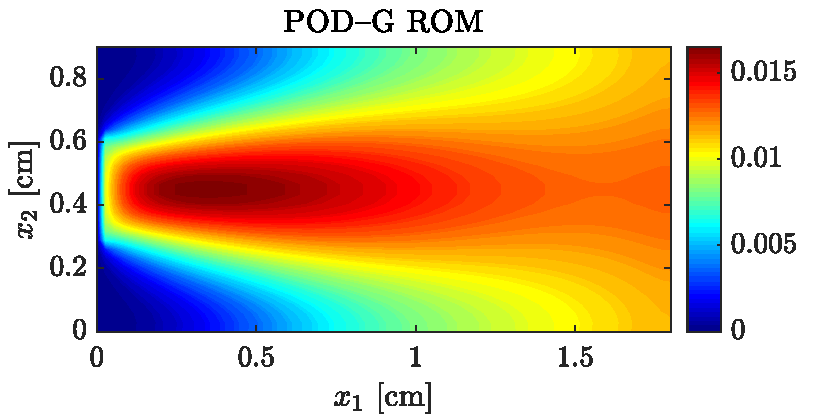
\includegraphics[width=\columnwidth]{GROM_T_param1.pdf}%
		\caption{Modèle réduit avec la méthode linéaire POD.}
		\label{fig:POD_ROM}
	\end{subfigure}\hfill
	\begin{subfigure}[t]{0.465\textwidth}
		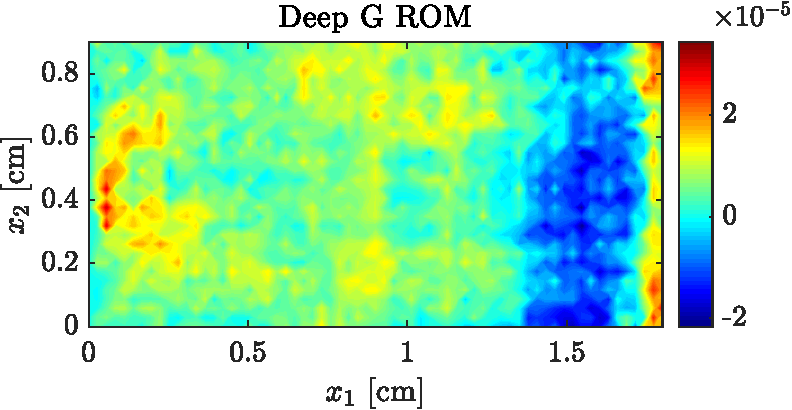
\includegraphics[width=\columnwidth]{DGROM_T_param1.pdf} 
		\caption{Modèle réduit avec réseaux des neurones.}
		\label{fig:DG_ROM}
	\end{subfigure}
	\caption[]{Réduction de modèle pour un problème de convection-diffusion-réaction. En utilisant un réseaux neuronaux convolutifs pour générer une variété non linéaire l'erreur associé à la réduction est drastiquement réduit par rapport à la méthode POD (de $10^{-2}$ à $10^{-5}$). Reproduit de \cite{lee2020} avec permission.}%
	\label{fig:deepROM}%
\end{figure}


\subsection{Lot de travaux}
Le projet est divisé en trois lots de travaux :

\begin{enumerate}
	\item Développement d'algorithmes numériques haute-fidélité pour des problèmes d'interactions fluide-structures basée sur le formalisme port-Hamiltonien et les élément finis en calcul extérieur.
	\item Méthodes de réduction garantissant le respect de la structure physique générés en utilisant les réseaux des neurones. 
	\item Utilisation des modèles réduits pour l'optimisation et comparaison avec les  modèles haute-fidélité.
\end{enumerate}

Chaque macro-tâche est directement associ\'ee \`a une thèse. 


\paragraph{\large WP1 : méthodes numériques pour systèmes couplés fluide-structure\\
Résponsable: Andrea Brugnoli et Doctorant 1\\}

La formalisation des problème fluide-structure au sein du formalisme port-Hamiltonien à été formalisé in \cite{califano2021energetic}. Pourtant, ce type d'interconnexion suppose que la partie mécanique soit représenté par un corps rigide. Dans ce premier lot de travail, on cherche à obtenir des modèles couplés d'interaction fluide-structure dans le cas où la partie structurelle est considérer déformable. Une fois que ces modèles seront dérivées, le focus principal de ce lot sera de générer des chemins numériques pour la préservations de la structure Hamiltonien à l'aide de la méthode à éléments finis en calcul extérieur. Cette tache représente un véritable défi computationnelle, spécialement si on cherche à résoudre le cas plus général possible d'interaction fluide-structure où la partie mécanique est très flexible et effectue des mouvements rigides. On pourra alors diviser la tache en considérant des problèmes de complexité croissante. 
\begin{enumerate}
	\item Si la structure est encastrée et les déformations sont petits, prenez par exemple une aile d'avion en conditions nominaux, on peut utiliser un maillage fixe au cours du temps. Ceci est du au fait que on peut utiliser les équations linéaire pour l'élasticité. 
	\item Si la structure peut bouger d'une manière rigide mais les déformations restent petit, par exemple dans le cas des turbomachine, des approches existent pour limiter la complexité des équations.
	\item Dans le cas le plus général, les équations de l'élasticité doivent être utilisés.
\end{enumerate}
Le doctorant choisi pour cette thèse devra alors concevoir des méthodes numériques capable de s'adapter à cette complexité croissante. La première défi portera à la résolution du premier cas, qui ne demandera pas d'introduire des technique spéciales pour modifier le maillage. Au contraire le cas successifs devront utiliser des méthodes pour considérer les déplacement du corps élastique (comme par exemple la méthode de frontières immergées \cite{peskin2002}).


\begin{figure}[h!]
	\begin{center}
		\begin{ganttchart}[y unit title=0.6cm,
			y unit chart=0.6cm, 
			x unit=0.4cm,
			vgrid,hgrid, 
			title label anchor/.style={below=-1.6ex},
			title left shift=.05,
			title right shift=-.05,
			title height=1,
			progress label text={},
			bar height=0.7,
			group right shift=0,
			group top shift=.6,
			group height=.4]{1}{30}
			%labels
			\gantttitle{Dur\'ee totale}{30} \\
			\gantttitle{$T_0 + 12$}{6} 
			\gantttitle{$T_0 + 24$}{6} 
			\gantttitle{$T_0 + 36$}{6} 
			\gantttitle{$T_0 + 48$}{6} 
			\gantttitle{$T_0 + 60$}{6} \\
			%tasks
			\ganttbar{Partenariats}{1}{2} \\
			\ganttbar{Code SCRIMP}{1}{1} \\
			\ganttbar{1$^\circ$ th\`ese}{4}{21} \\
			\ganttbar{2$^\circ$ th\`ese}{10}{27} \\
			\ganttbar{3$^\circ$ th\`ese}{13}{30} \\
			\ganttbar{Post-Doc}{16}{27} \\
			\ganttbar{Soutenances}{22}{30} \\
			\ganttbar{Dissémination}{28}{30} 
			%relations 
			\ganttlink{elem0}{elem2} 
			\ganttlink{elem1}{elem2} 
			\ganttlink{elem1}{elem3} 
			\ganttlink{elem1}{elem4} 
			\ganttlink{elem1}{elem5}
			\ganttlink{elem2}{elem5}
			\ganttlink{elem3}{elem5}
		\end{ganttchart}
	\end{center}		
\end{figure}


\subsection{Moyens et partenariats}
Pour ce que il concerne la mise en place du projet, des différents partenariats en France et \`a l'international seront mis en place. Pour ce qui concerne les aspect théoriques fondamentaux Bernhard Maschke (Universit\'e de Lyon), Arjan van der Schaft (University of Groningen) et Stefano Stramigioli (University of Twente) constitueront les interlocuteurs académiques principaux. \\

Pour ce qui concerne la première macro-tâche, il sera possible de prolonger le travail effectué dans le cadre de ma thèse, qui a donn\'e lieu a un code de calcul pour application multiphysique (le code SCRIMP décrit dans~\cite{brugnoli2021num}). Ce code sera ultérieurement développé pour traiter des problèmes d'interaction fluide-structure. Pour ce qui concerne la préservation de la physique au sein des algorithmes, des collaborations avec Marc Gerritsma (département d'aérodynamique de l'Universit\'e de Delft) et Herbert Egger (Johannes Kepler University Linz) seront mises en place. Pour ce qui concerne l'interaction fluide-structure, l'office National d'Études et de Recherches Aérospatiales (ONERA), garant d'une profonde expertise en ce domaine, représentera l'interlocuteur principal pour les problèmes liés au couplage multiphysique. 
\\


Pour ce qui concerne la deuxième macro-tâche, i.e. la réduction des modèles, il sera possible de mettre en place des collaboration avec Charles Poussot-Vassal (chercheur principal \`a l'ONERA),  Volker Mehrmann (TU Berlin) et George Haller (ETH Zurich). \\

Pour la troisième partie, il sera important de dialoguer avec Joseph Morlier (ISAE-Supa\'ero et Institut Clément Ader).

\subsection{Le projet MORPHEUS}


\section{Aspects innovants du projet et verrous scientifiques}





\subsection{Verrous scientifiques}


Le premier défi du projet consiste à implémenter des méthodes numériques pour la résolution des systèmes couplés multiphysiques. Ces modèles numériques devront retenir les propriétés physiques du problème (conservation d’énergie globale, traçage des échanges d’énergie entre les différents sous-systèmes, conservation d’invariants du problème). Dans l'industrie habituellement, des méthodes différentes sont utilisées pour simuler des physiques distinctes. Par conséquent, le couplage numérique ne représente pas correctement les flux d’énergie. L’utilisation d’un paradigme de modélisation unifié permettra donc d’effectuer les couplages de manière à respecter la physique. \\

Le second challenge du projet consiste à intégrer des techniques issues de l’Intelligence
Artificielle, qui seront utilisées pour obtenir des modèles réduits. Une technique très prometteuse en ce sens est présentée dans \cite{lee2020}, mais ici le respect des lois physiques est imposé a posteriori au travers de contraintes et non pas inclus au niveau de la structure de départ. Dans \cite{sun2020physics} des réseaux de neurones, entraînés pour minimiser l’erreur par rapport au bilan de masse et de la quantité de mouvement, sont utilisés pour s’affranchir de la simulation haute fidélité. Pourtant, cela ne garantit pas le respect de la structure physique et pose des soucis au niveau de l’interprétabilité des résultats. Conserver la structure physique de la simulation haute fidélité dans la représentation réduite permettra d’intégrer des outils d’intelligence artificielle d’une façon interprétable. \\

Le dernier objectif consistera à utiliser ces modèles réduits pour optimiser le design
mécanique des structures, et vérifier la validité des modèles réduits. Cette étape permettra
d’évaluer la validité et l’efficacité des modèles réduits par rapport aux simulations fines.
Typiquement dan l'industrie l’optimisation et les études paramétriques sont effectuées sur les
modèles fins, mais cela comporte des investissement considérables en termes de temps et de
ressources de calcul. Les modèles réduits seront plus rapides mais inévitablement
moins précis par rapport aux simulations fines. Venir à bout de ces trois macro-tâches
permettra de mieux comprendre le compromis entre temps de calcul et précision pour des
applications d’intérêt industriel. 

\subsection{Domaines d'application}


\begin{figure}[t]
	\begin{subfigure}[t]{0.3\textwidth}
		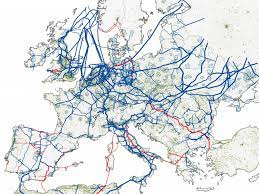
\includegraphics[width=\columnwidth]{EU_gas_network.jpeg}%
		\caption{Réseau européen du gaz (\href{https://vividmaps.com/the-european-natural-gas-network/}{Lien source})}
		\label{fig:network}
	\end{subfigure}\hfill
	\begin{subfigure}[t]{0.35\textwidth}
		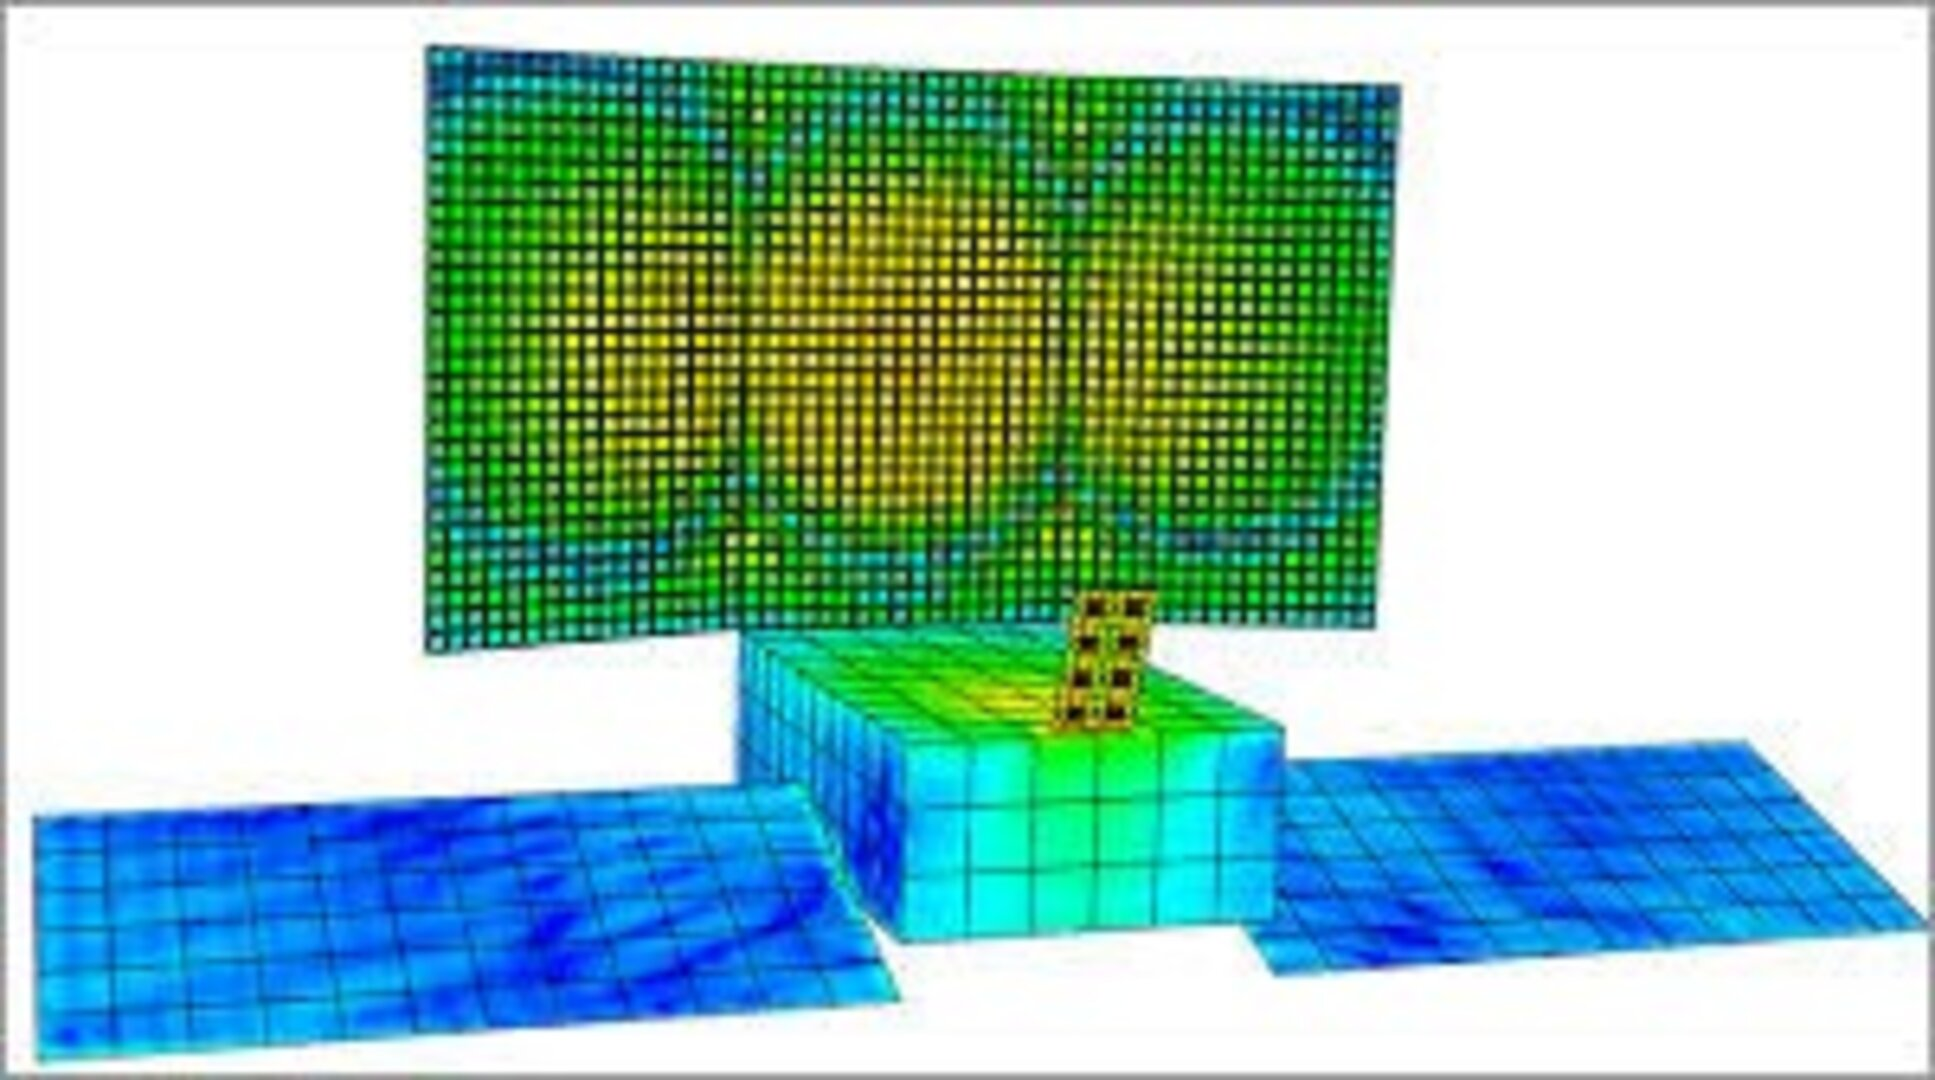
\includegraphics[width=\columnwidth]{Reflectarray.jpg} 
		\caption{Logiciel simulation antenne reflectarray (\href{https://www.esa.int/Enabling_Support/Space_Engineering_Technology/Smart_design_of_flat_reflectarray_satellite_antennas}{Lien source})}
		\label{fig:array}
	\end{subfigure}\hfill
	\begin{subfigure}[t]{0.25\textwidth}
		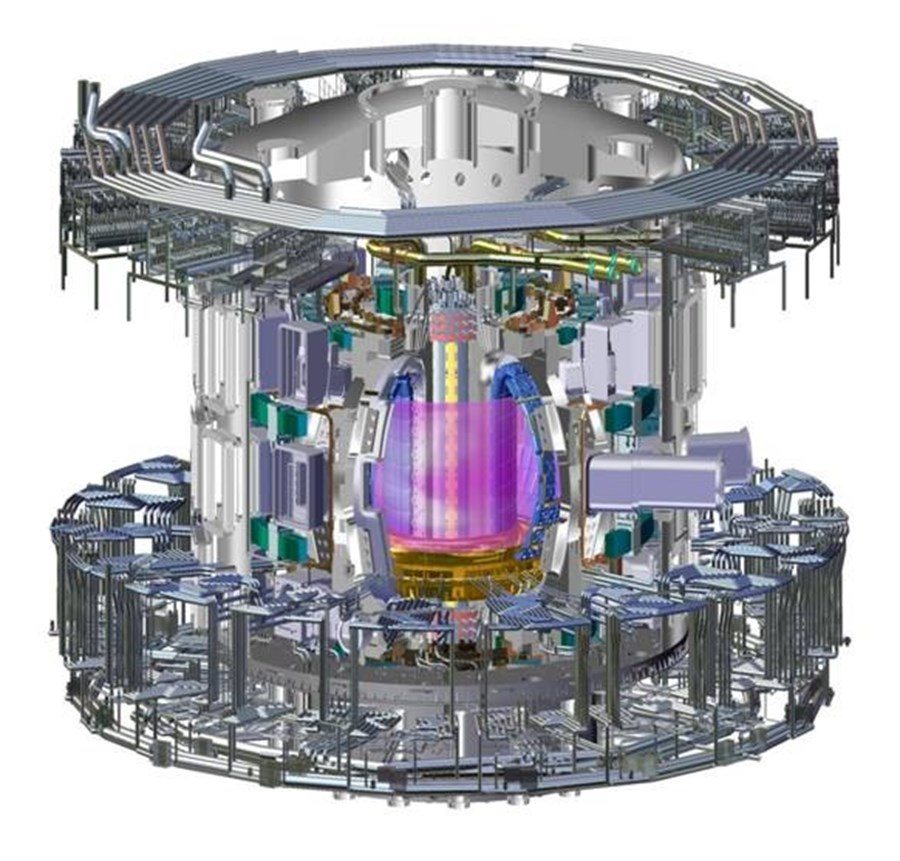
\includegraphics[width=\columnwidth]{tcws.jpg}%
		\caption{Le réacteur du projet ITER (\href{https://www.iter.org/newsline/-/1119}{Lien source})}
		\label{fig:sofi-mit}
	\end{subfigure}
	\caption[]{Exemple de cas d’application des outils computationels développés dans le cadre du projet MORPHEUS.}%
	\label{fig:applications}%
\end{figure}

Au-delà de l’aéronautique, où l’aéroélasticité et le design des turbomachines restent un challenge essentiel, différents secteurs d’applications pourront bénéficier des outils développés
dans le cadre de ce projet (cf. Fig \ref{fig:applications}): \\
\begin{itemize}
	\item Pour réduire les coûts associés à la maintenance des réseaux de distribution (énergie
	électrique, gas, hydrogène ou hydraulique), des méthodes structurées capables de représenter une hiérarchie de modèles sont nécessaires. Le coût de calcul est trop élevé pour pouvoir optimiser ces modèles directement.
	\item Afin de fournir des services Internet dans des endroits sans accès haut débit, une
	solution prometteuse consiste à utiliser des constellations de satellites équipés d'antennes constituées de différents modules réflecteurs (reflectarray). Pour concevoir ces modules, des modèles intégrant l’électromagnétisme et la thermomécanique sont nécessaires.
	\item  La production d’énergie à partir de la fusion nucléaire pose énormément de défis
	technologiques, à cause des conditions extrêmes de fonctionnement pour le réacteur. La fusion nucléaire représente un cas typique de problème multiphysique, où la dynamique des fluides interagit avec l’électromagnétisme d’une manière complexe.
\end{itemize}



\subsection{Portée du projet}

Les outils capables de prédire le comportement des systèmes complexes ont une importance
fondamentale pour nous aider à affronter les prochains défis technologiqes et sociétaux. Le fait que cette année le Prix Nobel de Physique ait été attribué à trois chercheurs travaillant sur ce sujet\footnote{\url{https://www.nobelprize.org/prizes/physics/2021/summary/}} confirme
l’importance et l’actualité de cet axe de recherche. Disposer d'outils quantitatifs performants pour traiter et comprendre la complexité qui nous entoure contribue :

\begin{enumerate}
	\item à faciliter le design des technologies opérantes, et à les pousser dans conditions extrêmes
	(avions très flexibles, turbomachines, fusées, etc.);
	\item à prévenir les risques dus au vieillissement des infrastructures, bâtiments (l’usure
	des matériaux introduit des non-linéarités);
\end{enumerate} 

Le fait d’utiliser un outil de modélisation unifié représente une nouveauté essentielle de ce projet.
Cela pourra permettre la création d’une infrastructure commune pour les outils numériques à la base de la digitalisation,  et donc faciliter son adoption dans l'industrie.



\subsection{Budget}
\begin{center}
\begin{tabular}{|c|c|}
	\hline
	D\'epense & Co\^{u}t \\
	\hline
	Porteur du projet (temps plein) & $5\times 60000=300000$ \\
	3 doctorants (temps plein) & $3\times 3\times 40000=360000$  \\
	1 Post-Doc (temps plein) & $2\times 55000=110000$ \\
	Personnels ISAE & $100000$ \\
	Matériel  et calcul HPC & $60000$ \\
	Frais annexes (conférences, workshops) & $60000$ \\
	\hline
	\textbf{Total} & 1000000 \\
	\hline
\end{tabular}
\end{center}



\footnotesize
\bibliographystyle{unsrt}
\bibliography{biblio_dossierLL}


\end{document}
